\section{Desenvolvimento do Software}

A metodologia adotada combina fundamentos da engenharia química com técnicas modernas de desenvolvimento de \textit{software}, visando garantir precisão nos cálculos e acessibilidade por meio de uma interface \textit{web} intuitiva. O projeto foi estruturado em etapas que abrangem desde o levantamento bibliográfico das equações de dimensionamento até a implementação e validação do sistema completo. O desenvolvimento foi dividido em quatro partes principais: \textit{backend}, \textit{frontend}, \textit{deploy} e versionamento.

\subsection{\textit{Backend}}

O \textit{backend} foi desenvolvido em \textit{Python}, utilizando o \textit{framework} \textit{FastAPI}, escolhido por sua alta \textit{performance}, suporte a tipagem forte e facilidade na criação de APIs RESTful. Essa camada é responsável por processar os cálculos, gerenciar as rotas de comunicação (\textit{endpoints}) e servir os resultados ao \textit{frontend}. Além disso, por se tratar de uma linguagem de alto nível, sua sintaxe é simples e intuitiva para iniciantes.

A Tabela \ref{tab:backend_libs} resume as principais bibliotecas e \textit{frameworks} utilizados, sua funcionalidade e a correspondência com aplicações típicas da engenharia química.

\begin{longtable}{|>{\raggedright\arraybackslash}p{0.2\textwidth}|>{\raggedright\arraybackslash}p{0.35\textwidth}|>{\raggedright\arraybackslash}p{0.35\textwidth}|}
\caption{Bibliotecas e \textit{frameworks} utilizados no \textit{backend}}
\label{tab:backend_libs} \\
\hline
\textbf{Nome} & \textbf{Funcionalidade} & \textbf{Como se enquadra no uso da Engenharia Química} \\ \hline
\endfirsthead
\caption[]{Bibliotecas e \textit{frameworks} utilizados no \textit{backend} (continuação)} \\
\hline
\textbf{Nome} & \textbf{Funcionalidade} & \textbf{Como se enquadra no uso da Engenharia Química} \\ \hline
\endhead
\hline
\multicolumn{3}{r}{\footnotesize{(Continua na próxima página)}} \\
\endfoot
\hline
\multicolumn{3}{c}{\footnotesize Fonte: Autoria própria.}
\endlastfoot
FastAPI & Framework web moderno para criação de \textit{APIs RESTful} em Python, com validação automática de dados e documentação interativa. & \textit{Backend} para expor os cálculos de engenharia química através de \textit{endpoints} HTTP, permitindo que a interface web ou outros sistemas acessem as funções de dimensionamento, balanço de massa, cálculos de reatores etc. \\ \hline
\textit{Uvicorn} & Servidor ASGI para executar aplicações \textit{web} assíncronas em \textit{Python}. & Executa o servidor da \textit{API FastAPI}, processando as requisições dos cálculos. \\ \hline
\textit{Pydantic} & Biblioteca para validação de dados e gerenciamento de configurações usando \textit{Python} \textit{type hints}. & Valida os dados de entrada dos cálculos (vazões, temperaturas, pressões, propriedades físicas etc.), garantindo que os parâmetros fornecidos estejam no formato e tipo corretos antes de executar os cálculos. \\ \hline
\textit{CoolProp} & Biblioteca especializada em propriedades termodinâmicas de fluidos, com banco de dados extenso de substâncias. & Cálculo de propriedades termodinâmicas (densidade, viscosidade, entalpia, entropia, calor específico etc.) de compostos e misturas. \\ \hline
\textit{Pint} & Gerenciamento de unidades físicas, conversões e cálculos dimensionais & Permite trabalhar com diferentes sistemas de unidades, garantindo consistência dimensional nos cálculos. \\ \hline
\textit{Matplotlib} & Biblioteca de visualização de dados e criação de gráficos 2D/3D. & Gera gráficos de processos químicos como curvas de reação, perfis de temperatura, diagramas de fases, curvas de bomba, e visualizações de resultados de simulações. \\ \hline
\textit{NumPy} & Biblioteca fundamental para computação científica com \textit{arrays} multidimensionais e operações matemáticas vetorizadas & Realiza cálculos matriciais, interpolações, operações vetoriais para balanços de massa e energia, resoluções de sistemas de equações lineares em processos químicos \\ \hline
\textit{SciPy} & Conjunto de algoritmos científicos para otimização, integração numérica, álgebra linear, estatística & Resolução de EDOs, otimiza processos químicos, realiza integrações numéricas para cálculos de conversão, ajuste de curvas experimentais \\ \hline
\textit{Pytest} & \textit{Framework} de testes, com suporte a testes unitários, testes de integração, \textit{fixtures}, parametrização e relatórios detalhados. & Permite validar automaticamente a confiabilidade dos cálculos de engenharia química, garantindo que equações, modelos matemáticos e rotinas numéricas estejam corretos e continuem funcionando após alterações no código. \\ \hline
\end{longtable}

\subsection{\textit{Frontend}}

O \textit{frontend} corresponde à interface gráfica do usuário, sendo a parte visual e interativa do sistema, acessada diretamente pelo navegador. Ele é responsável por exibir os resultados dos cálculos, receber dados de entrada e enviar as informações ao servidor (\textit{backend}).

Para consolidar uma base técnica mais robusta e sustentável, o \textit{frontend} foi estruturado sobre \textit{React} com \textit{Next.js} e \textit{TypeScript}. Essa combinação permite organizar a interface em componentes reutilizáveis, rotas e estados previsíveis, além de incorporar tipagem estática entre a camada visual e os contratos da API. Em vez de concentrar a lógica em arquivos monolíticos de \textit{JavaScript}, cada módulo passa a ser modelado como uma composição de componentes e serviços tipados, o que reduz acoplamento e favorece manutenção, testes automatizados e expansão futura.

No nível de interface, adotou-se \textit{Tailwind CSS} para composição visual utilitária e uma camada de componentes acessíveis baseada em primitivas modernas. Elementos antes supridos por \textit{plugins} legados, como campos de seleção enriquecidos, podem ser representados por componentes de \textit{combobox}/\textit{select} acessíveis, enquanto bibliotecas de ícones modulares, como \textit{Lucide}, oferecem consistência visual com baixo custo de manutenção. A renderização matemática por \textit{KaTeX} foi preservada por continuar adequada ao contexto didático do projeto. A Figura \ref{fig:piping_interface} ilustra a interface de usuário desenvolvida para o módulo de Piping, evidenciando as escolhas de \textit{design} descritas.

Na versão final do \textit{frontend}, a experiência foi reorganizada como um painel educacional único, com navegação lateral persistente, página inicial orientada por trilhas de aprendizagem e módulos de simulação agrupados por domínio. A interface passou a destacar, de forma explícita, o propósito pedagógico de cada área para estudantes e docentes, incorporando também uma visualização de escoamento inspirada no comportamento do número de Reynolds, indicadores compactos e cartões de contexto para reduzir a fricção na entrada da ferramenta.

\begin{figure}[H]
    \centering
    \caption{Interface gráfica do módulo de cálculos de tubulação (\textit{Piping})}
    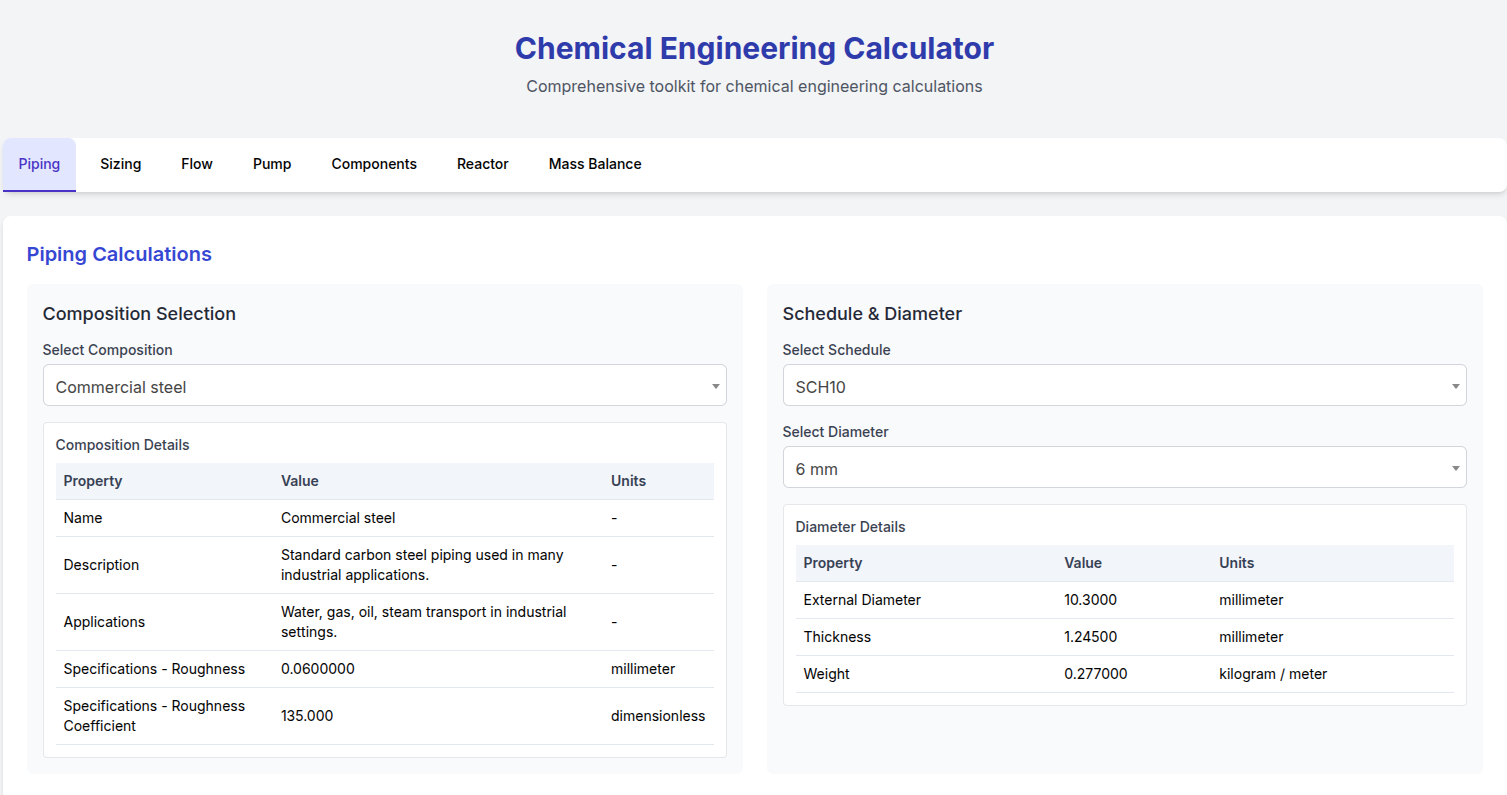
\includegraphics[width=\linewidth]{media/piping_interface.png}
    \fonte{Autoria própria.}
    \label{fig:piping_interface}
\end{figure}

\begin{table}[H]
\centering
\caption{Bibliotecas e \textit{frameworks} utilizados no \textit{frontend}}
\label{tab:frontend_libs}
\begin{tabular}{|>{\raggedright\arraybackslash}p{0.2\textwidth}|>{\raggedright\arraybackslash}p{0.7\textwidth}|}
\hline
\textbf{Nome} & \textbf{Funcionalidade} \\ \hline
\textit{React} & Biblioteca declarativa para composição de interfaces em componentes reutilizáveis e encapsulados. \\ \hline
\textit{Next.js} & \textit{Framework} para aplicações \textit{React} com empacotamento moderno, roteamento, otimização de \textit{build} e base adequada para evolução do produto. \\ \hline
\textit{TypeScript} & Superset tipado de \textit{JavaScript} utilizado para formalizar contratos de dados, reduzir erros de integração e melhorar manutenção. \\ \hline
\textit{Tailwind CSS} & \textit{Framework} utilitário que facilita a criação de interfaces responsivas e personalizadas com classes pré-definidas de estilo. \\ \hline
\textit{shadcn/ui} ou componentes baseados em Radix UI & Conjunto de componentes acessíveis e modulares para formulários, diálogos e seletores avançados, substituindo abordagens legadas baseadas em \textit{plugins}. \\ \hline
\textit{Lucide} & Biblioteca de ícones vetoriais modulares para navegação, estados visuais e ações contextuais na interface. \\ \hline
\textit{KaTeX} & Biblioteca \textit{JavaScript} para renderização rápida de equações em \LaTeX{} diretamente no navegador. \\ \hline
\end{tabular}
\fonte{Autoria própria.}
\end{table}

Além da pilha principal, a interface utiliza uma camada de componentes visuais próprios para o contexto da Engenharia Química, incluindo cartões de módulo, painéis didáticos, blocos de métricas e um visual de Reynolds para apoiar a leitura de escoamento, o que torna a navegação mais explicativa sem alterar o contrato com a \textit{API}.

\subsection{\textit{Deploy}}
O \textit{deploy} do sistema foi realizado por meio de \textit{Docker}, tecnologia que permite empacotar a aplicação e suas dependências em contêineres portáteis e reprodutíveis. Essa abordagem elimina problemas de compatibilidade entre ambientes e facilita o uso do \textit{software} em diferentes sistemas operacionais.

Foram criadas imagens separadas para o \textit{backend} e o \textit{frontend}, que podem ser executadas em conjunto ou individualmente. No caso da interface, a estratégia de empacotamento deixa de tratar apenas um conjunto estático de arquivos e passa a contemplar uma aplicação moderna compilada, preservando a possibilidade de distribuição independente da API. O uso do \textit{Docker} também simplifica futuras implementações em servidores remotos e integração com orquestradores, garantindo escalabilidade e isolamento dos serviços. A aplicação encontra-se disponível para acesso público em \url{https://tcc.homelab.sistemasj.com.br}.

\subsection{Versionamento}
O controle de versão foi implementado com o \textit{Git} para rastrear alterações no código-fonte, permitir colaboração e garantir segurança no desenvolvimento. O repositório foi criado no \textit{GitHub} como público, permitindo a colaboração entre diferentes contribuidores. O uso de versionamento também favorece a rastreabilidade científica do projeto, assegurando transparência e reprodutibilidade dos resultados obtidos. O repositório original pode ser acessado em \url{https://github.com/joao-baza/TCC}.
